% =========================================================================
% Secao 5 - Heterogeneidade socioeconomica
% =========================================================================

\section{Heterogeneidade socioeconômica}
\label{sec:heterogeneidade}

Esta seção explora as desagregações que são, à data desta nota,
inviáveis com os dados publicados pelo INEP, pois o Censo Escolar
não tem renda domiciliar nem raça do aluno individualizada nas
tabelas agregadas oficialmente divulgadas. Os números desta seção
referem-se à média 2018--2023, excluindo 2020 e 2021 para evitar o
ruído COVID, no painel inter-ano da PNADC sob a metodologia v5
descrita na Seção~\ref{ssec:definicoes}. A
Figura~\ref{fig:heterog_combined} consolida as desagregações por
sexo, raça, quintil de renda e defasagem idade-série, em quatro
painéis. Discutimos a seguir os achados centrais. Tabelas
desagregadas detalhadas estão no Apêndice~\ref{app:uf}, e figuras
adicionais nas Figuras~\ref{fig:het_sexo}--\ref{fig:het_regiao}.

\begin{figure}[htbp]
\centering
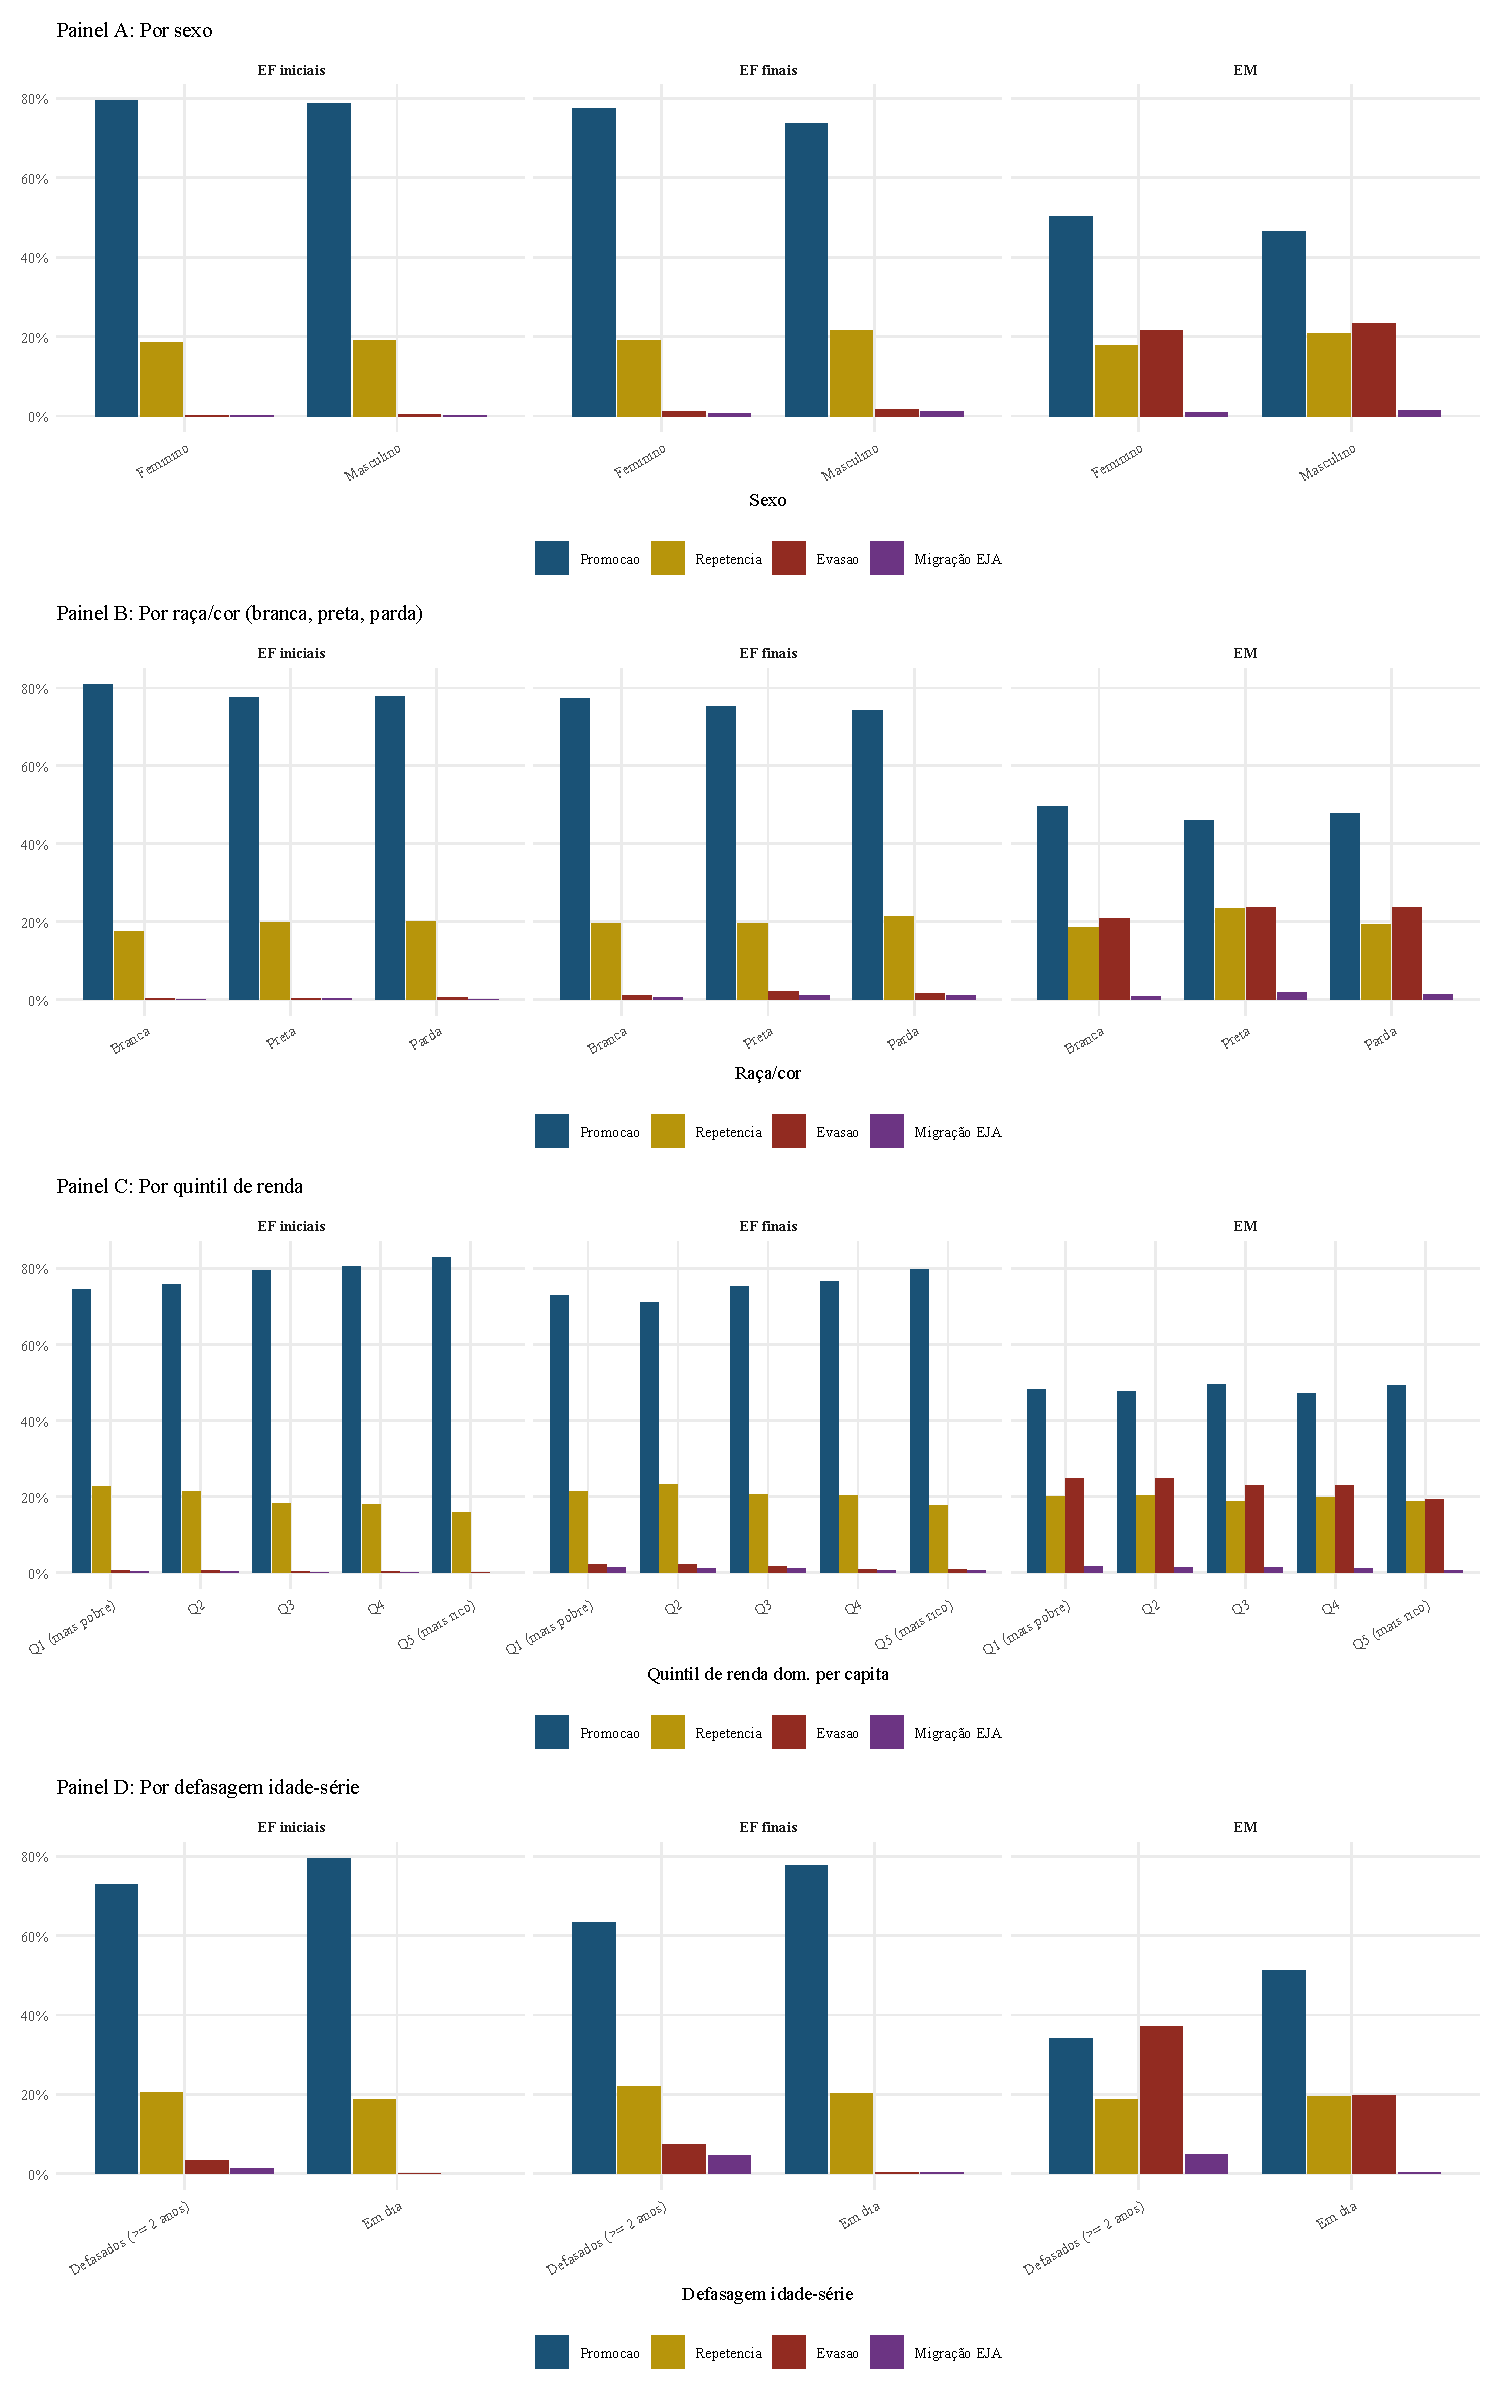
\includegraphics[width=0.95\textwidth]{../DataWork/5_Figures/output/F8_heterog_combined.pdf}
\caption{Taxas de fluxo escolar por dimensão socioeconômica, Brasil,
média 2018--2023 (ex-COVID).}
\label{fig:heterog_combined}
\figurenote{Universo: painel inter-ano da PNADC, com referência em
$t$ e $t+1$ tomadas entre $Q_2$ e $Q_3$ usando o máximo do nível
educacional. Cada painel reporta as quatro taxas (promoção,
repetência, evasão, migração para EJA) por dimensão.}
\end{figure}

A defasagem idade-série é o preditor mais forte de fluxo escolar
desfavorável no painel. A tabela detalhada
(Tabela~\ref{tab:distorcao}, no Apêndice~\ref{app:uf}) reporta as
taxas condicionais ao aluno iniciar o painel com defasagem de
pelo menos dois anos em relação à idade-padrão, comparadas às
taxas dos alunos em dia. As diferenças são substanciais. No EF
iniciais, os alunos defasados têm promoção de 73,0\%, contra
79,5\% dos alunos em dia, e evasão de 3,3\%, contra 0,1\%. No EF
finais, a promoção cai de 77,6\% para 63,2\%, e a evasão sobe de
0,4\% para 7,3\%. No EM, a diferença é dramática. A promoção cai
de 51,2\% para 34,0\%, e a evasão sobe de 19,6\% para 37,1\%, ou
seja, quase o dobro. A taxa de migração para EJA também cresce
muito entre os defasados, chegando a 4,9\% no EM, contra 0,3\%
para alunos em dia. Esse achado replica diretamente o padrão
documentado por \citet{Fernandes2011_atratividade} usando dados
mensais da PME, em que o abandono escolar concentra-se
desproporcionalmente entre alunos defasados, e estende-o ao
período contemporâneo com cobertura nacional. O resultado também
dialoga com \citet{SoaresAlvesFonseca2021_trajetorias} sobre o
uso de trajetórias educacionais como medida agregada de qualidade
da educação básica e com \citet{AlvesSoares2013_contexto} sobre
desigualdades de contexto na efetivação das políticas
educacionais.

Mulheres apresentam consistentemente melhor desempenho em todos os
indicadores e em todas as macroetapas, em linha com a literatura.
A diferença é especialmente visível no EM, em que a promoção
feminina é de cerca de cinquenta e dois por cento contra cinquenta
por cento masculina, com repetência menor entre as mulheres e
evasão similar entre os sexos. O Painel A da
Figura~\ref{fig:heterog_combined} e a Figura~\ref{fig:het_sexo}
detalham esse padrão. Os fatores que levam à evasão no EM
brasileiro afetam ambos os sexos similarmente, mas a vantagem
feminina na progressão de série persiste.

\begin{figure}[htbp]
\centering
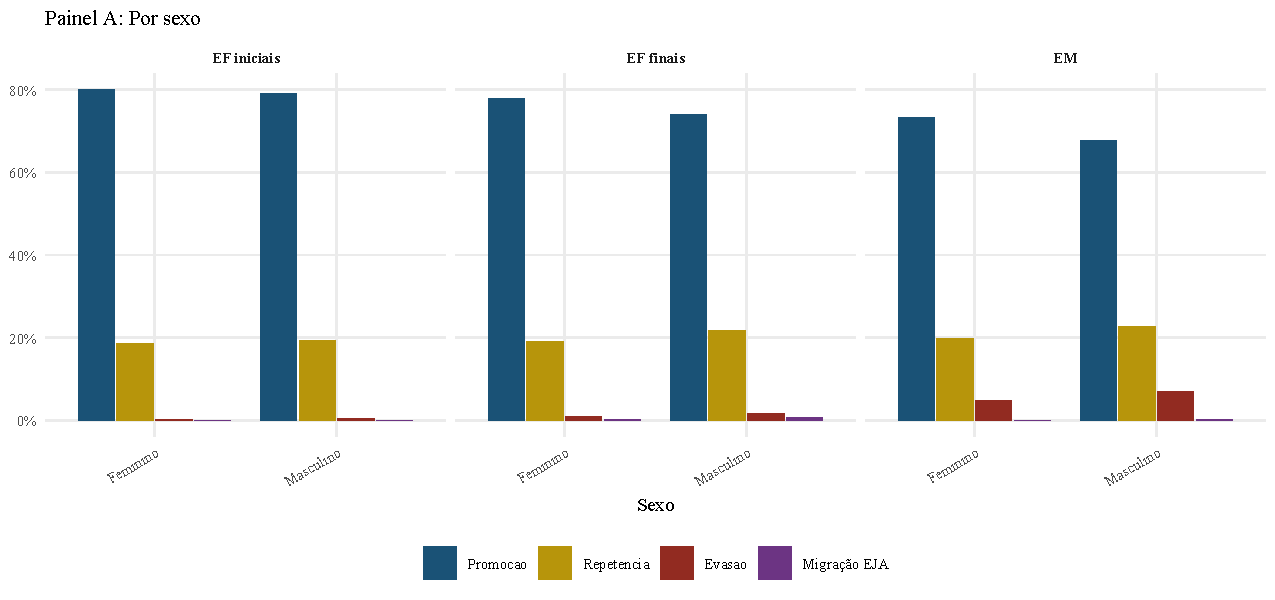
\includegraphics[width=0.95\textwidth]{../DataWork/5_Figures/output/F8a_heterog_sexo.pdf}
\caption{Taxas de fluxo escolar por sexo e macroetapa, média
2018--2023 (ex-COVID).}
\label{fig:het_sexo}
\end{figure}

O gradiente racial é consistente com a literatura recente de
estratificação educacional brasileira. Alunos pretos e pardos
apresentam promoção menor e evasão maior do que alunos brancos
em todas as macroetapas, com a diferença mais pronunciada no EM.
A Figura~\ref{fig:het_raca} reporta as quatro taxas por categoria
racial.

\begin{figure}[htbp]
\centering
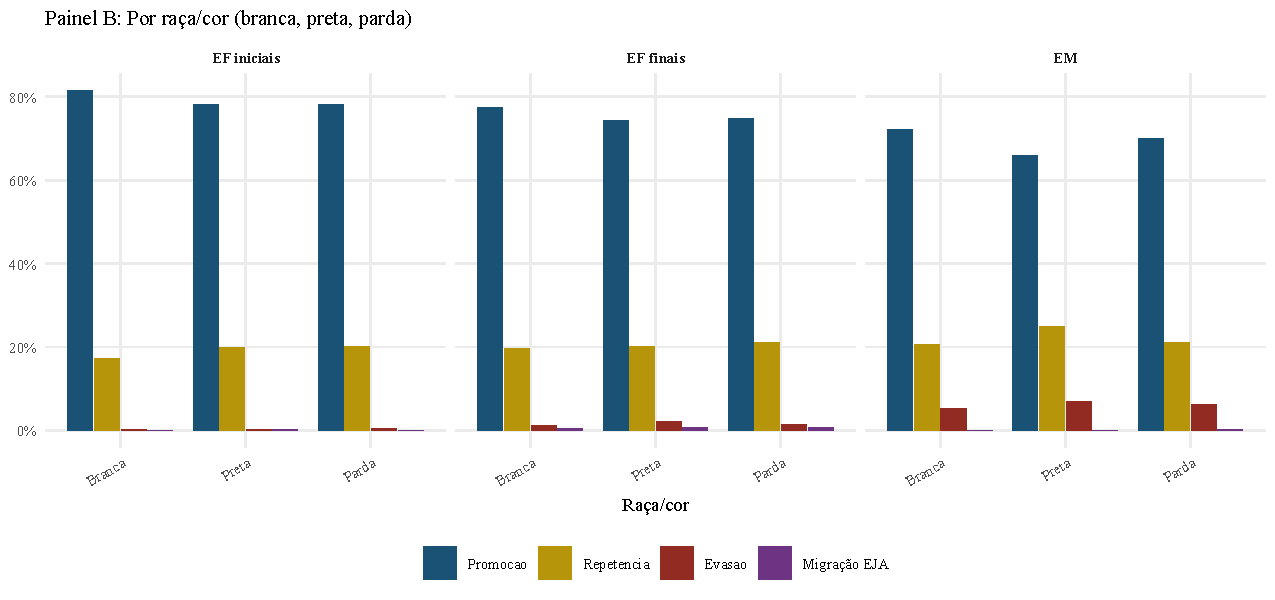
\includegraphics[width=0.95\textwidth]{../DataWork/5_Figures/output/F8b_heterog_raca.pdf}
\caption{Taxas de fluxo escolar por raça/cor e macroetapa, média
2018--2023 (ex-COVID).}
\label{fig:het_raca}
\end{figure}

O gradiente de renda é diferente entre EF iniciais e EM. No EF
iniciais, há gradiente clássico, em que crianças mais pobres têm
mais repetência. No EM, contudo, os desafios de retenção e
progressão afligem o sistema como um todo, e o gradiente de
renda perde intensidade. Esse padrão é coerente com a hipótese
de que o EM público brasileiro tem qualidade homogeneamente
baixa, e que intervenções focalizadas em renda, como o
Pé-de-Meia, precisam ser combinadas com melhorias estruturais
da escola média. A Figura~\ref{fig:het_renda} detalha por
quintil de renda domiciliar per capita.

\begin{figure}[htbp]
\centering
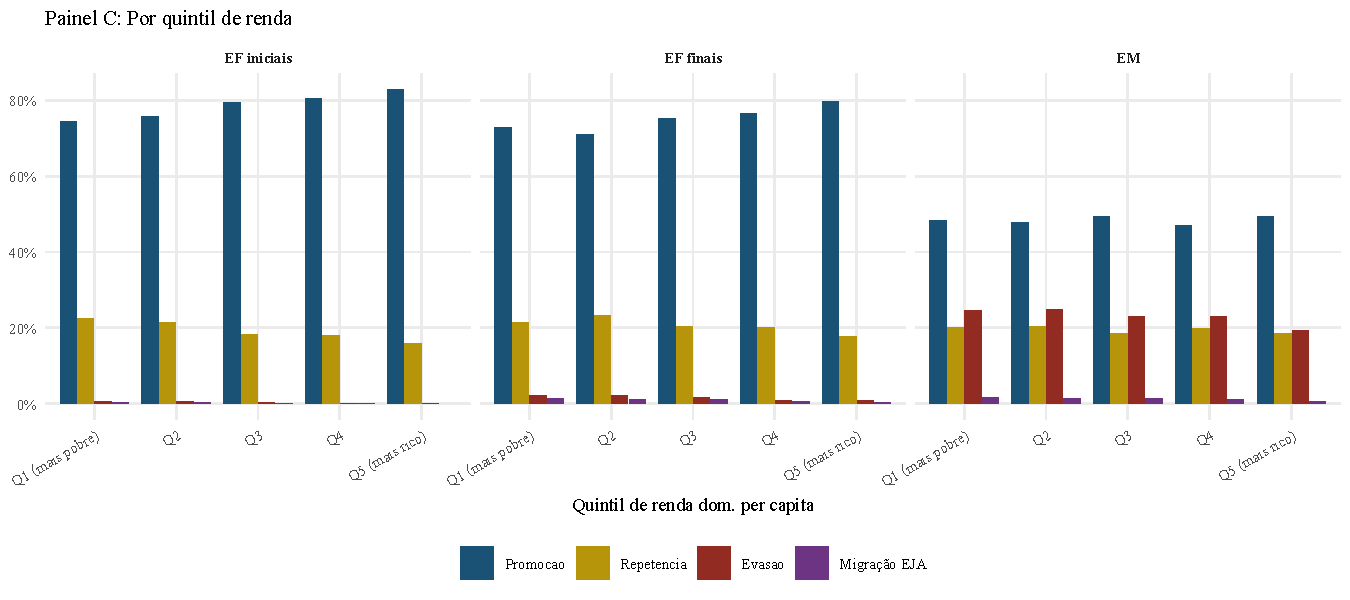
\includegraphics[width=0.95\textwidth]{../DataWork/5_Figures/output/F8c_heterog_renda.pdf}
\caption{Taxas de fluxo escolar por quintil de renda domiciliar
per capita e macroetapa, média 2018--2023 (ex-COVID).}
\label{fig:het_renda}
\end{figure}

A diferença entre rede pública e rede privada é grande,
especialmente no EM. Alunos da rede privada apresentam taxa de
promoção significativamente maior e taxa de evasão
significativamente menor do que alunos da rede pública. O
diferencial é parcialmente explicado pela composição
socioeconômica das duas redes, mas persiste mesmo após o
controle por renda observado na Figura~\ref{fig:het_renda}, o
que sugere a presença de um efeito-escola além do efeito-renda
sobre o fluxo educacional. A Figura~\ref{fig:het_rede} detalha
o gradiente por rede.

\begin{figure}[htbp]
\centering
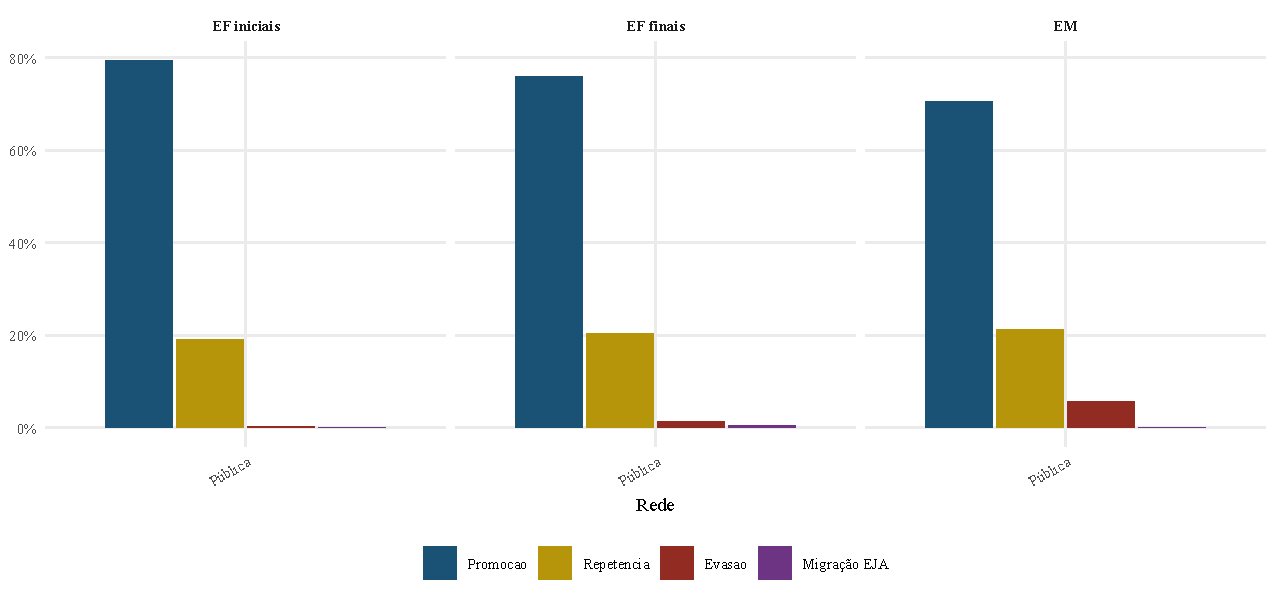
\includegraphics[width=0.95\textwidth]{../DataWork/5_Figures/output/F8e_heterog_rede.pdf}
\caption{Taxas de fluxo escolar por rede (pública/privada) e
macroetapa, média 2018--2023 (ex-COVID).}
\label{fig:het_rede}
\figurenote{Rede pública agrupa federal, estadual e municipal.
Rede privada inclui escolas particulares contratuais. A
composição socioeconômica das duas redes é diferente; ver
Apêndice para distribuição por quintil de renda.}
\end{figure}

A distribuição regional dos indicadores reflete o quadro de
desigualdades historicamente documentado no sistema educacional
brasileiro. As regiões Norte e Nordeste apresentam taxas de
evasão mais elevadas e taxas de promoção menores do que as
regiões Sudeste, Sul e Centro-Oeste, particularmente no EM. O
diferencial regional, mostrado na Figura~\ref{fig:het_regiao},
opera em conjunção com os demais gradientes (renda, raça,
defasagem) e é parcialmente atribuível à composição
socioeconômica, mas há também um componente regional residual
que aponta para diferenças de infraestrutura escolar e de
oportunidades locais.

\begin{figure}[htbp]
\centering
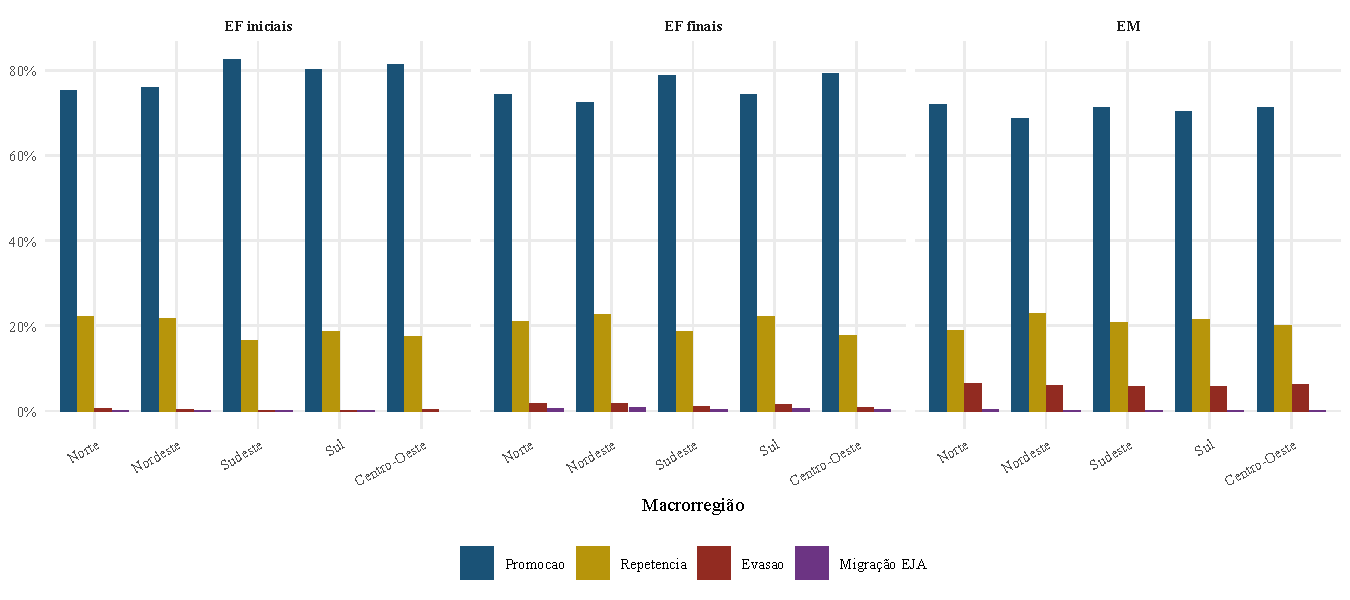
\includegraphics[width=\textwidth]{../DataWork/5_Figures/output/F11_heterog_regiao.pdf}
\caption{Taxas de fluxo escolar por macrorregião e macroetapa,
média 2018--2023 (ex-COVID).}
\label{fig:het_regiao}
\end{figure}

A Figura~\ref{fig:het_def} sintetiza visualmente a comparação
entre alunos em dia e defasados, confirmando que a defasagem é
o eixo de heterogeneidade com maior efeito sobre o fluxo, em
todas as macroetapas.

\begin{figure}[htbp]
\centering
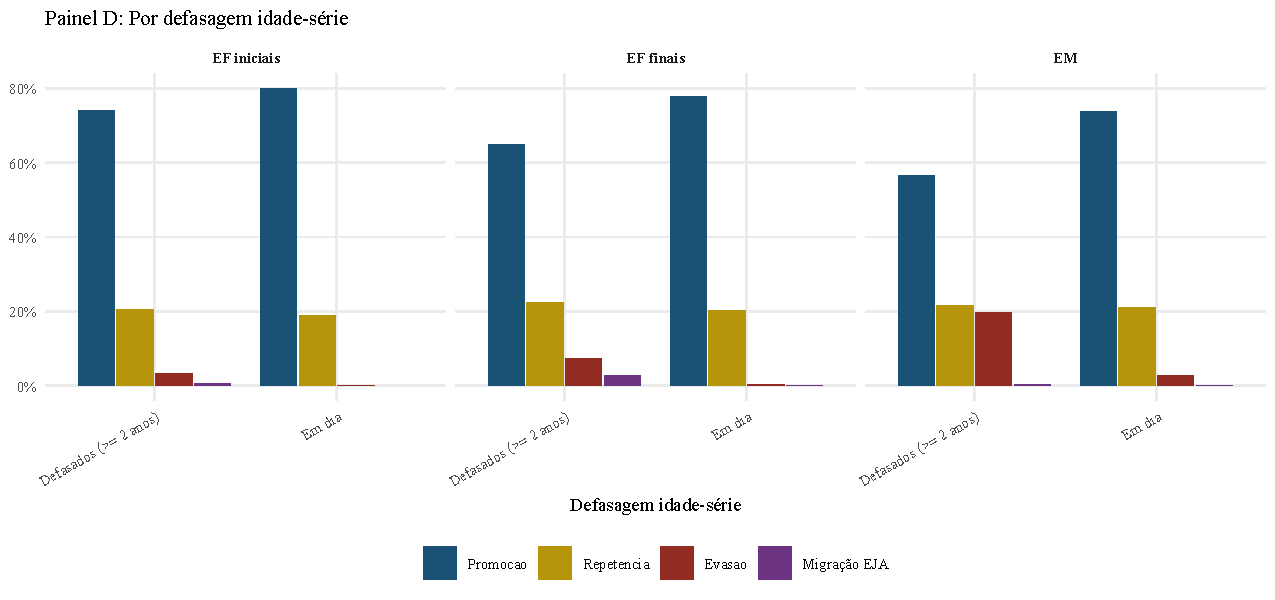
\includegraphics[width=0.95\textwidth]{../DataWork/5_Figures/output/F8d_heterog_defasagem.pdf}
\caption{Taxas de fluxo escolar por defasagem idade-série e
macroetapa, média 2018--2023 (ex-COVID).}
\label{fig:het_def}
\end{figure}

A leitura conjunta das seis dimensões de heterogeneidade
sugere uma hierarquia clara entre os preditores de evasão e de
não-progressão. A defasagem idade-série é dominante, em
particular no EM. A região e a rede aparecem em segundo plano,
refletindo a estrutura territorial e institucional do sistema.
Renda, raça e sexo, embora estatisticamente relevantes em
cortes univariados, estão parcialmente mediados pelas
dimensões anteriores, conforme apontado pela literatura de
\citet{SoaresAlvesFonseca2021_trajetorias} e
\citet{AlvesSoares2013_contexto}. A implicação para o desenho
de políticas é direta. Intervenções focalizadas apenas em
renda, como transferências condicionadas, tendem a ter efeito
limitado se não atacarem simultaneamente a defasagem
idade-série, que é o canal mais forte de risco de evasão. Esse
diagnóstico converge com a agenda de programas como o
Pé-de-Meia, que combinam transferência com mecanismos de
recuperação de aprendizagem.

Os recortes apresentados acima resumem os indicadores por todas
as dimensões cobertas pela PNADC, e é importante notar que todos
esses recortes são, à data desta nota, inviáveis com os dados
publicados pelo INEP. O Censo Escolar mais detalhado, em seus
microdados, tem identificador socioeconômico mínimo (rede,
dependência administrativa, localização urbana ou rural), mas
não tem renda domiciliar nem raça do aluno individualizada. A
diferença não é de método, mas de disponibilidade pública de
informação. Esse é o segundo argumento central pela
complementaridade entre PNADC e Censo Escolar.
